\section{Theorie}
\label{sec:Theorie}
In dem betrachteten Versuch wurden Biegeversuche an elastischen Metallstäben durchgeführt, um das Elastizitätsmodul der jeweiligen Materialien zu bestimmen.
\subsection{Spannung und Elastizitätsmodul}
Bei der Verbiegung der Stäbe greifen Kräfte an der Oberflläche der Stäbe an, welche zu Gestalts- und Volumenveränderungen führen können. Wenn man diese Kräfte auf die Fläche bezieht, erhält man die physikalische Größe der Spannung. Der senkrecht zur Oberfläche stehende Anteil der Spannung wird als Normalspannung /sigma bezeichnet und die oberflächenparallele Komponente heißt Tangential- oder Schubspannung. \newline
Bei Festkörpern kann oft ein linearer Zusammenhang zwischen der Spannung /sigma und der relativen Längenänderung $\frac{\Delta L}{L}$ beobachtet werden:
\begin{equation}
	\sigma = E \cdot \frac{\Delta L}{L}
	\label{eqn:1}
\end{equation}
\autoref{eqn:1} wird auch als Hookesches Gesetz bezeichnet. Die materialabhängige Konstante $E$ bezeichnet man als Elastizitätsmodul und soll in diesem Versuch ermittelt werden. Da es möglich ist, dass keine Messvorichtung zur Verfügung steht mit der es möglich ist die Längenänderung $\Delta L$ hinreichend genau zu messen, wurde im vorliegenden Versuch mit der Biegung eine Defomation genutzt, die eine leichter messbare Veränderung (die Messgröße D) am Stab hervorruft.

\subsection{Durchbiegung eines homogenen Stabes bei einseitiger Einspannung}
In \autoref{fig:1seitig} ist zu erkennen wie eine Gewichtskraft $F$ an einem einseitig eingespannten Stab mit Querschnitt $Q$ eine Durchbiegung $D(x)$ hervorruft. In der Abbildung ist die neutrale Faser, in der keine Spannungen oder Längenänderungen auftreten, gestrichelt angedeutet.
\begin{figure}
	\centering
	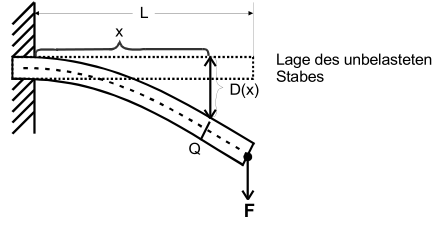
\includegraphics{durchbiegung_einseitig.PNG}
	\caption{Verbiegung eines Stabes bei einseitiger Einspannung \cite{sample}}
	\label{fig:1seitig} 
\end{figure}
Die Zug- und Druckspannungen, die an $Q$ angreifen, bewirken ein Drehmoment $M_\sigma$, das durch Integration über Q zu ermitteln ist: 

\begin{equation}
    M_\sigma = \int_Q y \sigma(y) \; \symup{d}q.
	\label{eqn:2}
\end{equation}
Dabei ist $y$ der Abstand des Flächenelements $\symup{d}q$ zur neutralen Faser.
Der Stab wird sich dann so verbiegen, dass die beiden Drehmomente an jeder Stelle x übereinstimmen:
\begin{equation}
    M_\sigma = M_F
	\label{eqn:3}
\end{equation}
Das Drehmoment $M_F$ wird durch die Kraft $F$ mit Hebelarm $(L-x)$ ausgelöst:
\begin{align}
    M_\sigma &=M_\text{F}  \\
    \iff \; \int_Q y \sigma(y) \; \symup{d}q &= F \cdot (L - x)
	\label{eqn:4}
\end{align}

Mit
\begin{equation}
    \sigma(y) = E y \frac{ \symup{d}^{ 2 }D }{ \symup{d}x^{ 2 } }	
\end{equation}

und \autoref{eqn:4} erhält man:
\begin{equation}
    E \frac{ \symup{d}^{ 2 }D }{ \symup{d}x^{ 2 } } \int_Q y^2 \; \symup{d} q =F(l-x)
	\label{eqn:5}
\end{equation}

Die Größe 

\begin{equation}
    \symbf{I} = \int_Q y^2 \; \symup{d} q(y).
    \label{eqn:traegheit}
\end{equation}
bezeichnet man als Flächenträgheitsmoment. Die Berechnung des Flächenträgheitsmoments wird in \autoref{sec:flaechentraegheitsmoment} beschrieben.

Nach Integration von \autoref{eqn:5} erhält man dann für die Durchbiegung D in Abhängigkeit vom Abstand x von der Einspannung:
\begin{equation}
    D(x) = \frac{F}{2 E \symbf{I}} \left(L x^2 - \frac{x^3}{3} \right) 
    \qquad (\text{für } 0 \leq x \leq L)
    \label{eqn:Biegung}
\end{equation}



\subsection{Durchbiegung eines homogenen Stabes bei zweiseitiger Auflage}
Wie in \autoref{fig:2seitig} zu sehen ist, greift beim beidseitig gelagerten Stab eine Gewichtskraft $F$ in der Mitte des Stabes an und verursacht eine Durchbiegung $D(x)$. Also greift die Kraft $F/2$ mit Hebelarm $x$ an der Querschnittsfläche $Q$ an.
\begin{figure}
	\centering
	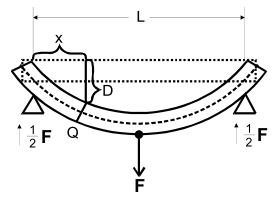
\includegraphics{durchbiegung_zweiseitig.PNG}
	\caption{Verbiegung eines Stabes bei zweiseitiger Auflage \cite{sample}}
	\label{fig:2seitig}
\end{figure}
Als Drehmomente für die beiden Stabhälften ergeben sich also: 
\begin{align}
    M_\text{F} &= - \frac{F}{2} x \qquad \qquad \; \; \,
    (\text{für } 0 \leq x \leq \frac{L}{2})\\
    M_\text{F} &= - \frac{F}{2} (L - x) \qquad (\text{für } \frac{L}{2} \leq x \leq L)
\end{align}

Mit \autoref{eqn:5} ergibt sich bei beidseitiger Auflage dann:
\begin{align}
    \frac{ \symup{d}^{ 2 }D }{ \symup{d}x^{ 2 } } &= - \frac{F x}{2 E \symbf{I}}  \qquad \qquad \; \; \,
    (\text{für } 0 \leq x \leq \frac{L}{2})\\
	\frac{ \symup{d}^{ 2 }D }{ \symup{d}x^{ 2 } } &= - \frac{F (L-x)}{2 E \symbf{I}} \qquad (\text{für } \frac{L}{2} \leq x \leq L)
\end{align}
Eine erste Integration dieser Gleichungen liefert:
\begin{align}
    \frac{ \symup{d}D }{ \symup{d}x } &= - \frac{F x^{2}}{4 E \symbf{I}} + C \qquad \qquad \qquad \; \; \,
    (\text{für } 0 \leq x \leq \frac{L}{2})\\
	\frac{ \symup{d}D }{ \symup{d}x } &= - \frac{F }{2 E \symbf{I}} (Lx - \frac{x^{2}}{2})+C´ \qquad (\text{für } \frac{L}{2} \leq x \leq L)
\end{align}

Mit der Randbedingung, dass die Tangente der Biegekurve in der Stabmitte ($x=L/2$) horizontal verläuft ($\frac{ \symup{d}D }{ \symup{d}x }=0$) kann man $C$ und $C´$ berechnen. 
\begin{align}
    C &= \frac{F L^{2}}{16 E \symbf{I}}  \\
    C´ &= \frac{3F L^{2}}{16 E \symbf{I}}  
    \label{eqn:c}
\end{align}

Einsetzen von $C$ und $C´$ und eine weitere Integration liefern dann für die Durchbiegung:

\begin{align}
    D(x) &= \frac{F}{48 E \symbf{I}} \left(3 L^2 x - 4 x^3 \right) 
    \qquad \qquad \qquad \qquad \: (\text{für } 0 \leq x \leq \frac{L}{2}) \\
    D(x) &= \frac{F}{48 E \symbf{I}} \left(4 x^3 - 12 L x^2 + 9 L^2 x - L^3 \right) 
    \qquad (\text{für } \frac{L}{2} \leq x \leq L)
    \label{eqn:beidseitig}
\end{align}


\subsection{Berechnung des Flächenträgheitsmoments}
\label{sec:flaechentraegheitsmoment}
Das Flächenträgheitsmoment $\mathbf{I}$ wird, da in dem Versuch nur runde Stäbe betrachtet wurden,
in Polarkoordinaten berechnet:
\begin{align}
	\mathbf{I} 
	&= \int_Q y^2 dq(y) 
	\\
	&= \int_0^{2\pi} d\varphi \int_0^r dr^\prime r^\prime 
	\left( r^\prime\sin(\varphi) \right)^2
	\\
	&= \frac{\pi}{4} r^4
\end{align}

\cite{sample}
